\documentclass[a4paper,11pt,oneside]{article}
% Add packages
\usepackage{graphics}	%NY
\usepackage{pifont}		%Symboler
\usepackage{afterpage}

\usepackage[T1]{fontenc}
\usepackage[utf8]{inputenc}
\usepackage[english,danish]{babel}
\usepackage{graphicx}
\usepackage{microtype}
\usepackage{lmodern}
\usepackage{lipsum}
\usepackage{makeidx} % Indexing package
\usepackage[intoc]{nomencl} % Nomenclature package
\usepackage{color}
\usepackage{mathpazo}
\usepackage[crop=pdfcrop]{pstool}
\usepackage{multirow}
\usepackage{textcomp}
%\usepackage[version=3]{mhchem}
\usepackage{relsize}
\usepackage{hyperref}
\usepackage{textpos}
\usepackage{indentfirst}
\usepackage{listings}
\usepackage{siunitx}
\usepackage{tikz}
\usetikzlibrary{shapes.geometric, arrows}
\usepackage[a4paper,left=3cm,right=3cm,top=3cm,bottom=3cm]{geometry}
\usepackage{wrapfig}
\usepackage{booktabs}
\usepackage{setspace}
\usepackage{mathptmx}
\usepackage{lmodern}
\usepackage{txfonts}
\usepackage{titlesec}
	\setcounter{secnumdepth}{4}

%\addto\captionsenglish{\renewcommand{\refname}{Litteraturliste}}
%\renewcommand{\bibname}{Litteraturliste}

\onehalfspacing

\setlength{\parindent}{1em}

\graphicspath{{pictures/}}

\everymath{\displaystyle}

% Avoid a warning
\pdfminorversion=5

\EndPreamble

%\usepackage{natbib} % Bibliography package
%\usepackage{siunitx} % Should stay after \EndPreamble

% Create a theorem environment
%\usepackage{amsthm}
\newtheorem{theorem}{Theorem}

\usepackage{xcolor,calc}

% Enable indexing
\makeindex

% Enable nomenclature
\makenomenclature

% Enable line numbering
%\usepackage{lineno}
%\pagewiselinenumbers
%\modulolinenumbers[5]

% Change table of contents name
\renewcommand*{\contentsname}{Table of Contents}

% Get a signature command
\makeatletter
\newcommand*{\getlength}[1]{\strip@pt#1}
\makeatother

\newlength{\signlength}
\setlength{\signlength}{0.5\textwidth}

\newcommand{\signature}[1]{%
\noindent \line(1,0){\getlength{\signlength}}\\
\noindent #1
}

% Add measuring units to nomenclature
\newcommand{\nomunit}[1]{\renewcommand{\nomentryend}{\hspace*{\fill}#1}}
\setlength{\belowcaptionskip}{10pt plus 5pt minus 5pt}

% Company logo
\def\bCompanyLogo{false}

% A fix for memoir-kluwer
\renewcommand{\bf}{\textbf}

% Set listings
\renewcommand\lstlistingname{Code snippet}
\renewcommand\lstlistlistingname{Code snippet}

\definecolor{white}{gray}{1.0}
\definecolor{light-gray}{gray}{0.95}
\definecolor{dkgreen}{rgb}{0,0.6,0}
\definecolor{gray}{rgb}{0.5,0.5,0.5}
\definecolor{mauve}{rgb}{0.58,0,0.82}

\lstset{
  frame=tb,
  language=C++,
  aboveskip=3mm,
  belowskip=3mm,
  showstringspaces=false,
  columns=flexible,
  basicstyle={\ttfamily},
  numbers=left,
  numberstyle=\tiny\color{gray},
  numbersep=11pt,                  
  stepnumber=1,                  
  captionpos = b,
  keywordstyle=\color{blue},
  commentstyle=\color{dkgreen},
  stringstyle=\color{mauve},
  backgroundcolor=\color{white},  
  breaklines=true,
  breakatwhitespace=true,
  tabsize=3,
  showspaces=false,
  showtabs=false
}



%Other setups

\usepackage{todonotes}
\graphicspath{{./pictures/}}
%\usepackage{amsmath}

\hypersetup{
    colorlinks,
    citecolor=green,
    filecolor=magenta,
    linkcolor=blue,
    urlcolor=cyan
}\hypersetup{
					colorlinks, 
					linkcolor={black},
					citecolor={blue!50!black},
					urlcolor={blue!80!black},
					}
\usepackage{fancyhdr}
\usepackage{lastpage}
\pagestyle{fancy}
\renewcommand{\sectionmark}[1]{\markright{\thesection.\ #1}}
\lhead{\korttitel}
\chead{}
\rhead{\rightmark}
\lfoot{\forfattere}
\cfoot{}
\rfoot{	\hfill \break
		\hfill \break
		Side \thepage \thinspace af \pageref{LastPage} \textbf{}}
\renewcommand{\headrulewidth}{0.5pt}
\renewcommand{\footrulewidth}{0.5pt}

\newcommand{\myparagraph}[1]{\paragraph{#1}\mbox{}\par}

\newcommand{\korttitel}{Tin Can Skype}
\newcommand{\forfattere}{
Anders Ellinge, 
Anders Fredensborg Rasmussen,
Daniel Holst Hviid,
Mathias Elbæk Gregersen
	\newline
Rasmus Skjerning Nielsen,
René Tidemand Haagensen,
Sarah Darmer Rasmussen
}

\begin{document}
%	\definecolor{ColorH1}{rgb}{0.212,0.373,0.569}
\definecolor{ColorH2}{rgb}{0.141,0.197,0.376}
\definecolor{ColorH234}{rgb}{0.310,0.506,0.741}
\definecolor{ColorOthers}{rgb}{0.141,0.247,0.376}
\definecolor{White}{rgb}{1, 1, 1}
\definecolor{Gray}{rgb}{0.5, 0.5, 0.5}

\thispagestyle{empty}

\begin{center}        % Centrerer teksten
  \Huge
  \color{ColorH2}
  \textbf{\textit{Tin Can Skype}} 					\\
  \huge
  \textbf{\textit{RB-MRO3 - Gruppe 3}} 				\\
  \vspace{10mm}
  \color{Gray}
  \normalsize
  \bfseries{Uddannelse og semester:} 				\\
  \Large
  \color{ColorOthers}
  \normalfont{\textit{Robotteknologi - 3. semester}}\\
  \vspace{6mm}
  \color{Gray}
  \normalsize
  \bfseries{Afleveringsdato:} 						\\
  \Large
  \color{ColorOthers}
  \normalfont{\textit{18. December 2015}} 			\\
  \vspace{6mm}
  \color{Gray}
  \normalsize
  \bfseries{Vejleder:} 								\\
  \Large
  \color{ColorOthers}
  \normalfont{\textit{Ib Refer (refer@mmmi.sdu.dk)}}\\
  \vspace{6mm}
  \color{Gray}
  \normalsize
  \bfseries{Gruppemedlemmer:} 						\\
  \Large
  \color{ColorOthers}
  \normalfont{\textit{
 Anders Ellinge (aelli14@student.sdu.dk) 					\\ 
 Anders Fredensborg Rasmussen (andra14@student.sdu.dk) 		\\
 Daniel Holst Hviid (dahvi14@student.sdu.dk) 				\\
 Mathias Elbæk Gregersen (magre14@student.sdu.dk) 			\\
 Rasmus Skjerning Nielsen (rasni14@student.sdu.dk) 			\\
 René Tidemand Haagensen (rehaa14@student.sdu.dk) 			\\
 Sarah Darmer Rasmussen (srasm14@student.sdu.dk)
  }} \\
  \vspace{12mm}
  \begin{figure}[ht]
	\centering
	
\includegraphics[scale=0.25]{pictures/svg2.pdf} 
  \end{figure}
  \vspace{8mm}
  \normalsize
  \textsl{Det Tekniske Fakultet} 					\\
  \textsl{Syddansk Universitet} 					\\   
\end{center}
%	\setcounter{page}{1}
%	\pagenumbering{arabic}
	\include{Forside/Forside}
\section{Abstract}
This project demonstrates how to create at chat application using C++. The computers using the application must be able to communicate with DTMF tones and a communication protocol must be dessigned.
The created application also includes a login and user history feature.
\newline
Agile software development, in partucular Scrum, has been used to simplify our project challenges by dividing them into smaller issues.
\newline
The created software is divided into layered softwarearchitecture by using datacommunication layers, such as the physical layer, the data link layer, the transportation layer and the application layer. Our main issues were solved by using: Goertzel for efficient tone recognition, CRC for error detection in data packages and Stop-and-Wait for establishing a connection between two processes.	
%	\section{Abstract}
This project demonstrates how to create at chat application using C++. The computers using the application must be able to communicate with DTMF tones and a communication protocol must be dessigned.
The created application also includes a login and user history feature.
\newline
Agile software development, in partucular Scrum, has been used to simplify our project challenges by dividing them into smaller issues.
\newline
The created software is divided into layered softwarearchitecture by using datacommunication layers, such as the physical layer, the data link layer, the transportation layer and the application layer. Our main issues were solved by using: Goertzel for efficient tone recognition, CRC for error detection in data packages and Stop-and-Wait for establishing a connection between two processes.
%	\pagebreak
%	\section{Forord}
Denne rapport er udarbejdet af gruppe 3, på andet semester på Civilingenør i Robotteknologi på Syddansk Universitet.
Rapporten er blevet skrevet i forbindelse med dette semesters projekt og beskriver hvordan denne gruppe har valgt at løse opgaverne i det valgte projekt, "Tin Can Skype", som er et chatprogram, der bruger DTMF-toner og indeholder bla. et simpelt log-in og historik system. 
\newline
Formålet med denne rapport er, at læseren skal være i stand til at læse og forstå projektet ved blot at have grundlæggende viden om C++ og datakommunikation, og ved at læse rapporten. 
\newline
\par
I forbindelse med dette projekt, blev følgende udstyr stillet til rådighed:
\begin{itemize}
	\item To mikrofoner
	\item To højtalere
\end{itemize}


%	\pagebreak
	
%	\tableofcontents
%	\pagebreak
	
	
%	\section{Indledning}
\subsection{Projektbeskrivelse}
I dette projekt er to højtalere og to mikrofoner blevet stillet til rådighed. Formålet med dette projekt er, at kunne sende data vha. DTMF-toner.
\newline
Det valgte projekt er et chatprogram, der udvikles i C++, og skal have de primære funktioner:
\begin{itemize}
	\item Overførsel af tekst.
	\item Log-in funktioner.
	\item Historik af chat-samtale.
\end{itemize}

Desuden er disse sekundære funktioner blevet overvejet:
\begin{itemize}
	\item Filoverførsel
	\item Gruppe chat
	\item Spil
	\item Redigering af tidligere beskeder
	\item Video streamings funktioner
	\item Humørikoner
\end{itemize}

Herudover er der desuden blevet overvejet at bruge en tredje computer, som kan bruges som en server.
Her vil mindst to computere altså være i stand til at kommunikere med hinanden vha. DTMF-toner.

\subsubsection{Krav til produktet}
Følgende krav blev stillet til projektet:
\begin{itemize}
	\item Bærbare computere skal kommunikere med hinanden, eller evt. et embedded system, ved	udveksling af lyd
	\item Der skal anvendes DTMF toner, og der skal designes en kommunikationsprotokol
	\item Der skal udvikles en distribueret applikation i C++
	\item Der skal anvendes en lagdelt softwarearkitektur
	\item Arkitekturen kunne være client/server med f.eks. tykke klienter
\end{itemize}
For at fuldføre dette projekt skal der anvendes to computere som skal være i stand til at kommunikere med hinanden ved hjælp af lyd i form af DTMF-toner. Derudover skal dette programmers i C++, her bruges klasser.

\subsubsection{Metodebeskrivelse}
Vi har i dette projekt valgt at benytte SCRUM, da alle gruppe medlemmer således er i stand til at arbejde med den metode der passer dem bedst. 
Vi har valgt at bruge brainstorm, som vores primære form for idégenererings-teknik.
Desuden prøver gruppen så vidt muligt at beregne alle de ting, der kan beregnes på forhånd.

\subsubsection{Afgrænsning}
Her ses de emner, som gruppen har overvejet at arbejde med. De primære funktioner er de funktioner som skal løses først, mens de sekundære løses efter tidsbegrænsning.
\newline
%Følgende punkter kan godt slettes hvis nødvendigt:
Primære funktioner:
\begin{itemize}
	\item Overførsel af tekst
		\subitem Protokol
		\subitem Karakter definition
		\subitem Størrelse
	\item Historik
		\subitem Tidspunkt
		\subitem Størrelse
	\item Log-in
\end{itemize}

Sekundære funktioner:
\begin{itemize}
	\item Fil-overførsel
		\subitem Protokol
		\subitem Queue
	\item Gruppe chat
		\subitem Protokol
	\item Spil database
		\subitem Protokol
		\subitem Funktion
	\item Rediger tidligere beskeder
		\subitem Protokol
		\subitem Funktion
	\item Stream funktion
		\subitem Protokol
		\subitem Funktion
	\item Humørikoner
		\subitem Char def.
		\subitem Database
	\item GUI
		\subitem Agil
	\item Sky "server"
		\subitem Funktion
\end{itemize}
%	\subsection{Workload (product backlog)}
Der laves en product backlog i stedet for en tidplan (se figur \ref{fig:workload}).
\begin{figure}[ht]
	\centering
	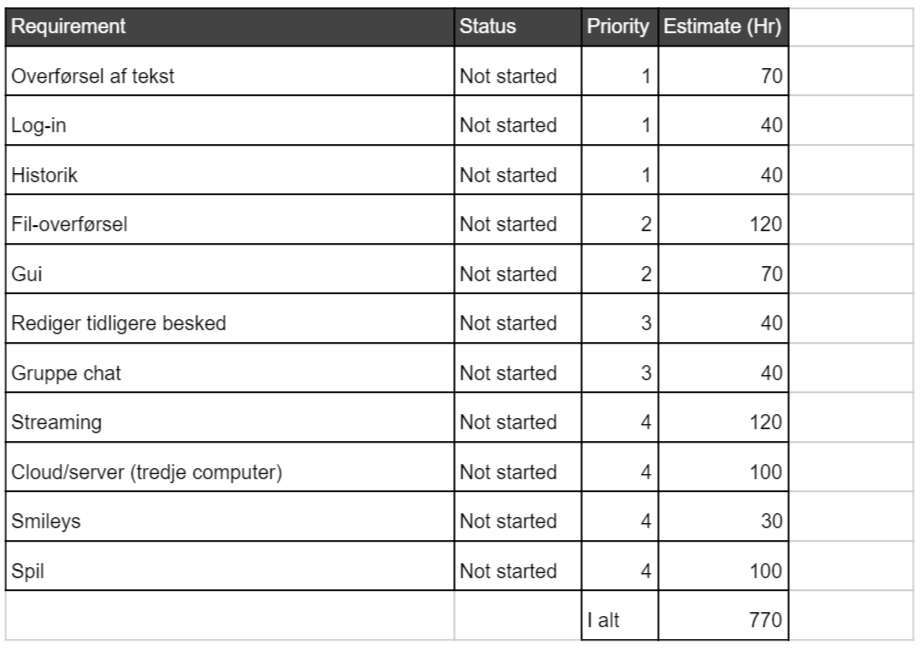
\includegraphics[width=15cm,height=25cm,keepaspectratio]{pictures/Workload.png}
	\caption{Product backlog}
	\label{fig:workload}
	\end{figure}
\newline
En product backlog er et værktøj inden for metoden SCRUM, som viser hvor langt tid en opgaver tager i mandetimer og hvilken status opgaven har (Not started, In process og Finished).

%	\pagebreak
	
%	\section{Softwareudvikling AKA Greger er dum}
\subsection{Projektstyring}
Under de første møder til projektet, blev det aftalt at projektet skulle planlægges ved hjælp af sprints fra Scrum og at der skulle holdes jævnlige Scrum møder.
\newline
Der blev i starten af projektet derfor lavet en product backlog, hvori der blev angivet over hvor lang tid, hver eneste funktionalitet ville tage at implementere. Denne product backlog kan ses i BILLAG.
\newline
Sprintene skulle defineres ud fra, hvad der vil skabe mest værdi for projektet. Denne planlægning var tiltænkt at man kunne tilpasse projektarbejdet i forhold til undervisningen bedre. Derudover skulle sprints også laves på baggrund, for først at løse kravene og derefter visse udvalgte sekundære funktionaliteter.
\newline
Efter en sprint var defineret, ville der blive oprettet en Sprint backlog, som skulle dokumentere hvor meget arbejde der blev lagt i en problemstilling, og hvor meget workload der var tilbage. Sprint backloggen skulle derfor opdateres løbende under den pågældende sprint Sprint backlog'en fra uge 47-49 kan ses i figur \ref{fig:4749}:
\begin{figure}[ht]
	\centering
	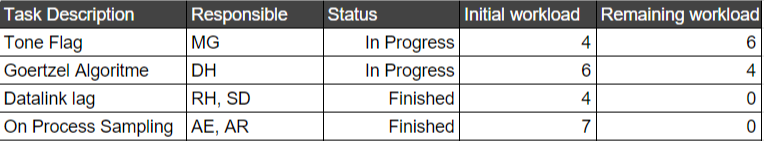
\includegraphics[width=15cm,height=25cm,keepaspectratio]{pictures/SprintBack47_49.png}
	\caption{Uge 47-49 sprint backlog}
	\label{fig:4749}
\end{figure}
\hfill \break

Yderlige eksempler på Sprint backlogs kan findes i BILAG.
\newline
Til Scrum møderne blev der udspecificeret en klar plan for, hvordan møderne skulle foregå, og hvilke elementer der skulle gennemgåes under møderne. I denne plan blev der også skrevet et kort teori afsnit, omkring hvordan man skal forholde sig til både Scrum møder og backlogs. Dette blev gjort med den hensigt, at hvert medlem ville være i stand til, at sikre at et Scrum møde blev udført korrekt og at backlogs blev opdateret.
\newline
Denne plan kan ses i BILLAG.

\subsection{Software Requirements Specification (SRS)}

\subsubsection{Idéudvikling}
Der blev i starten af projektet idéudviklet på den applikation der skulle laves. Der var flere idéer, hvorefter én blev valgt. Imellem disse idéer var en matematik applikation hvor en klient kunne sende et spørgsmål til en server og få et svar tilbage. Idéen var inspireret af Wolfram Alpha. Derudover var der også en idé, som til sidst blev valgt, som gik ud på at lave en chat applikation. Chat applikationen var inspireret af Skype, som fungerer på klient til klient plan. Der blev dog lagt op til at man kunne undersøge at lave en klient-server-klient hvis tiden var til det.
\hfill \break
Efter at have specificeret hvilken applikation der overordnet skulle laves, blev der lavet en brainstorm for krav til funktionaliteterne på applikationen, som kan ses på figur. 
\begin{figure}[ht]
	\centering
	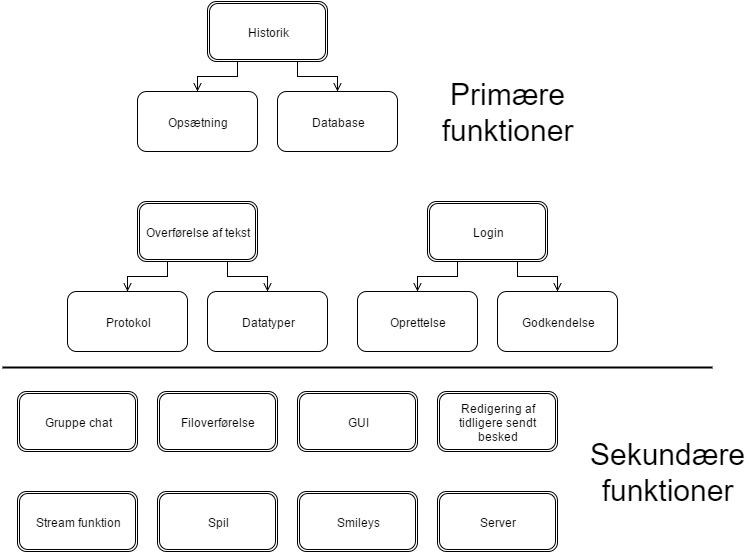
\includegraphics[width=15cm,height=25cm,keepaspectratio]{pictures/Ideudvikling.png}
	\caption{Brainstorm}
	\label{fig:brain}
\end{figure}
\newline
Som der ses på figur \ref{fig:brain} er funktionaliten delt op i to kategorier, primære- og sekundære funktioner. Hvor primære funktioner repræsenterer de funktionaliteter der minimum skal være i applikationen. De sekundære funktioner repræsenterer udvidelser som kan skabe værdi for brugeren.

\subsubsection{Kravspecifikation}
Udover at applikationen har nogle funktionaliteter, skal applikationen også have nogle krav. Disse krav er med til at opbygge applikationen og hjælper med at lede projektet mod en række problemstillinger der skal løses.
\newline
Kravene er som følger:
\begin{itemize}
	\item Sende beskeder mellem 2 applikationer
	\item Brugergrænseflade
	\item Pålidelig dataoverførsel
	\item Fejl testning af beskeder
	\item Se tidligere sendte og modtagede beskeder
	\item Login
\end{itemize}

\subsection{Softwareudvikling}
For at opbygge en velfungerende applikation,  er det imperativt at følge principperne indenfor softwareudvikling.

\subsubsection{Analyse fasen}
Der blev udarbejdet use cases, som viser hvordan brugeren interagerer med programmet, og som derudover hjælper til at afdække krav til applikation.
\newline
De use cases der blev udarbejdet var:
\begin{itemize}
	\item Login
	\item Historik
	\item Send besked
	\item Modtag besked
\end{itemize}
Use case over Send besked kan ses på figur HOMOSEXUEL og de resterende use cases kan findes i bilag BILLAG.
\hfill \break
Disse use cases blev brugt til at udarbejde en domænemodel, som kan ses i figur 
\begin{figure}[ht]
	\centering
	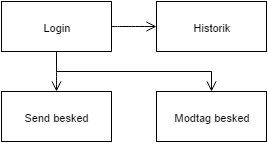
\includegraphics[width=10cm,height=10cm,keepaspectratio]{pictures/Domainmodel.png}
	\caption{Domænemodel}
	\label{fig:dom}
\end{figure}
\newline
Domæne modellen giver et simpelt indblik i hvordan applikationen skal fungere.
\hfill \newline
Udover at domæne modellen lægger op til at vi har som minimum fire klasser, blev det konstateret at der er behov for tre yderlige klasser, som opfylder følgende krav fra SRS, da de ikke blev afdækket af use casene: pålidelig dataoverførsel, brugergrænseflade og fejl testning af beskeder. Disse klasser blev midlertidigt navngivet \texttt{Fejlkontrol}, \texttt{UI} og \texttt{Levering}.

\subsubsection{Design klassen}
For at udarbejde et design klasse diagram blev der taget udgangspunkt i domænemodellen. Ved udvidelse og tilpasning af klasse diagrammet blev der anvendt design mønstre fra GRASP.
\newline
Jf. GRASP skal der være en controller, som er det første objekt efter en UI der modtager og koordinerer et systems operationer. Denne klasse bliver oprettet og snedigt kaldet Controller.
\newline
En skabelon for klasse diagrammet blev lavet, på baggrund af denne udvides og tilpasses den til et klasse diagram i en iterativ proces.
\begin{figure}[ht]
	\centering
	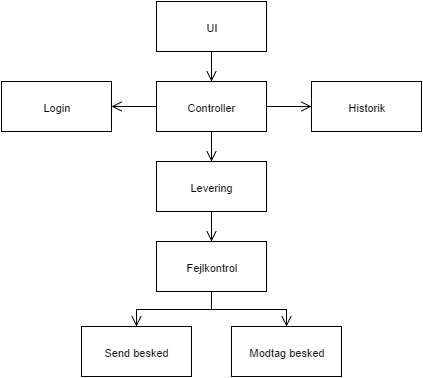
\includegraphics[width=10cm,height=10cm,keepaspectratio]{pictures/Flow.png}
	\caption{Flowmodel}
	\label{fig:flow}
\end{figure}
\newline
Under den iterative proces blev nogle meget generelle funktionaliteter undersøgt - hvordan man sender en besked og modtager en besked. Disse lagde op til nogle diskussioner og problemstillinger som diskuteres senere i rapporten. Grundet den iterative proces blev Send besked og Modtag besked omdybt til \texttt{Afspil} og \texttt{MyRecorder} for bedre at afspejle deres ansvarsområde. Jf. GRASPs principper havde disse klasser yderst lav kobling, men også lav cohesion grundet at der var mere ansvar i klasserne end de antydede. Derfor blev det konkluderet at disse ansvarsområder skulle deles op for at skabe højere cohesion. \texttt{Afspil} klassen havde ansvaret for at afspille toner, men ikke ansvaret for også at genererer toner. Derfor blev der lavet en information expert der påtog sig ansvaret at holde information omkring toner,netop klassen \texttt{Tone}. \texttt{MyRecorder} havde ligeledes kun et ansvar - at optage. Ansvaret for at analyserer optagelsen blev derfor tillagt en pure fabricated klasse ved navn \texttt{Goertzel}, for igen at øge cohesion.
\hfill \break

Senere i den iterative proces blev der draget inspiration fra datakommunikations lagdelte struktur - Open Systems Interconnection modellen (OSI). I denne model indgår der to lag, som afspejler klasserne Lervering- og Fejlkontrols ansvarsområde, nemlig: Datalinklaget(DLL) og Transportlaget. Klasse \texttt{Levering} er således blevet omdøbt til Transportlag, og \texttt{Fejlkontrol} er blevet omdøbt til \texttt{DLL}.
\newline
Grundet den iterative proces indeholdte DLL flere ansvarsområder end først forventet. Dette gjorde at man også her var nødsaget til at opdele ansvarsområdet. Der blev derfor pure fabricated en klasse, som ydede en service til DLL. Denne klasse fik navnet \texttt{CRC}, baseret på dens service.
\hfill \break
Disse udvidelser på klasse diagrammet skabte en ny problemstilling, de forskellige klasser snakker ikke i samme data format. Dataformaterne der snakkes i, er char strings, bit strings og tone chars.
\newline
Derfor blev der indført to klasser baseret over adapter pattern princippet, hvis formål var at oversætte dataformatet mellem de forskellige klasser. Adapter klasserne blev kaldt \texttt{CharDefinition} og \texttt{Tonekonvertering}.
\hfill \break
Efter projektets sidste iteration endtes der ud med et klasse diagram der kan ses på næste side.
\afterpage{\null\newpage}
%	\input{subsections/TeoriSWU}
	
%	\input{subsections/Praksis}
%	\subsubsection{Domænemodel}
%	\input{subsubsection/Designklasse}
	
%	\section{Det Fysiske Lag}
\subsection{Teori}

%	\subsection{Fysisk Lag Ind}
dsf
\newline
dkdk idkfgfdggfd
%	\subsubsection{Teori}
\underline{\textbf{Send-and-Wait protokol}}
\newline
Stop-and-Wait er et special tilfælde af Go-Back-N.
Stop-and-Wait har to sekvensnumre, mens Go-Back-N har flere
\newline
Ved hjælp af sekvensnummerering af pakkerne, er modtageren i stand til at konstatere om den modtagne pakke er den korrekte, eller om den har et forkert nummer i forhold til rækkefølgen.
\newline
Automatic repeat request (ARQ) benyttes når mistede eller fejlbehæftede pakker skal retransmitteres. Pakker retransmitteres hvis en ny ACK ikke er modtaget inden timeren udløber.
\newline

\textbf{Open} %En tel af TCP
\newline
Udføres når både sender og modtager er aktive.
\newline
Som der ses i figur \ref{fig:open}, sendes Segment 0, når Sender er aktiv. Hvis Modtager er aktiv oprettes der forbindelse og Modtager sender ACK 0 (acknowledgement 0) og Sender ved at der er forbindelse.
\newline
Hvis Modtager derimod ikke er aktiv vil Sender ikke modtage ACK 0, og Sender vil derfor vente 10 sekunder før igen at sende Segment 0. Dette vil Sender gøre op til tre gange, hvis nødvendigt.
\begin{figure}[ht]
	\centering
	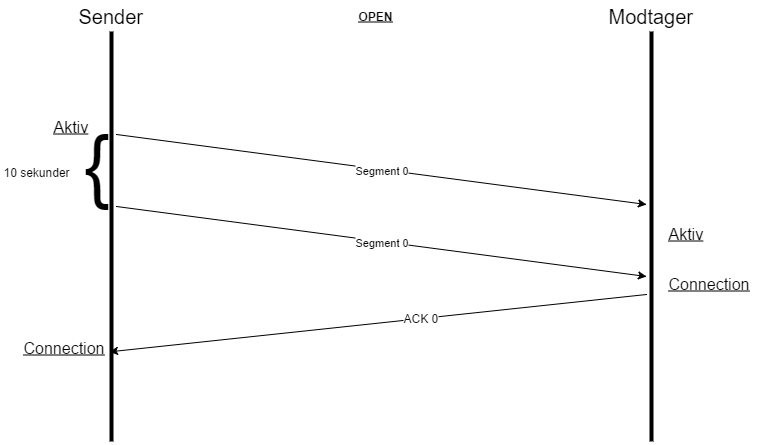
\includegraphics[width=10cm,height=20cm,keepaspectratio]{pictures/Open.png}
	\caption{Open}
	\label{fig:open}
\end{figure}

\hfill \break
\textbf{Stream} %En del af TCP. Der laves ingen Stream. Ingen model, mere teori.
\newline
Stream delen, som kan ses på figur \ref{fig:stream}, er den del hvor data sendes.
\newline
Her sender Sender først Segment 1. Hvis dette er blevet korrekt modtaget vil Modtager sende ACK 1.
Dette vil forstætte indtil Close. 

\begin{figure}[ht]
	\centering
	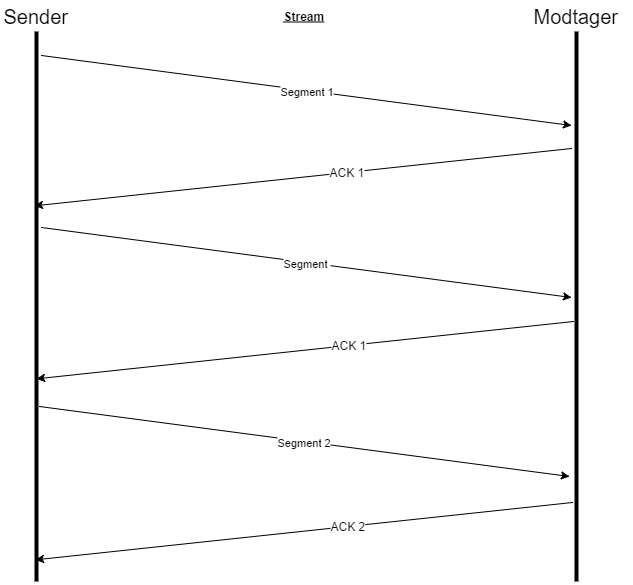
\includegraphics[width=10cm,height=20cm,keepaspectratio]{pictures/Stream.png}
	\caption{Stream}
	\label{fig:stream}
\end{figure}
\textbf{Close}
\newline
Close delen kan ses på figur \ref{fig:close}.
\newline
I denne del gør Sender Modtager opmærksom på at der ikke sendes mere.

\begin{figure}[ht]
	\centering
	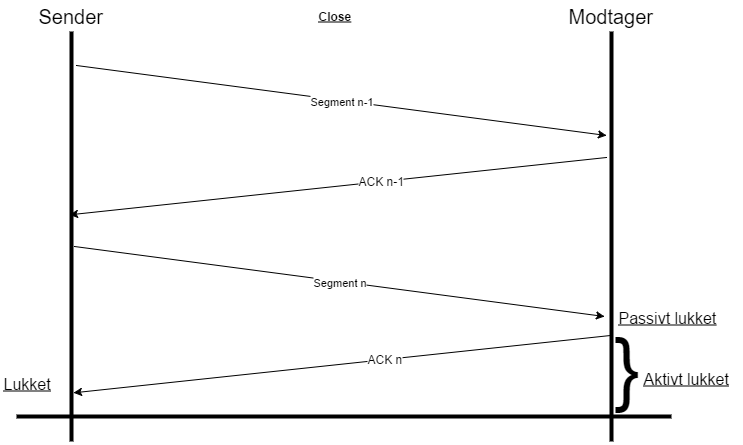
\includegraphics[width=10cm,height=20cm,keepaspectratio]{pictures/Close.png}
	\caption{Close}
	\label{fig:close}
\end{figure}

\hfill \break
\hfill \break
\hfill \break
\hfill \break
\underline{\textbf{Flag}}
\newline
I projekt koden er der benyttet tre flag til at fortælle om beskeden er en probe, accept, eller sidste besked.
Der benyttes 3 bit, til at definere flaget. 001 er probe, 010 er accept og 100 er last.
%	\subsubsubsection{Goertzel}
sdf
%	\input{subsubsections/ProgrammeringDFLInd} %Med kodeeksempler
%	\input{subsections/FysiskLagUd}
%	\input{subsubsections/TeoriDFLUd}
%	\subsection{Programmering} %Med kodeeksempler
	
	
%	\section{Data Link Laget}
%	\subsection{Teori}
\underline{\textbf{CRC}}
\newline
CRC står for Cyklisk Redundant Check, og bruges til fejl-detektering.
Formålet med fejl-detektering er at gøre det muligt for modtageren at afgøre om et datagram, sendt gennem en støjet kanal, er blevet beskadiget.
For at gøre dette konstruer senderen en checksum og føjer denne til datagrammet.
Modtageren er i stand til at bruge CRC til at beregne checksum af det modtagne datagram og sammenligne denne med den vedlagte checksum for at se, om datagrammet er blevet modtaget korrekt.\cite{ross}
%CRC er i stand til at detektere og korrigere fejl i sekvenser af bits, og kan derfor bruges i datatransmission samt i datalagring, for at beskytte filer fra fejl.
\newline
CRC er baseret på polynomiel aritmetik, primært beregning af resten når et polynomium divideres med et andet. Addition og subtraktion udføres ved hjælp af modulo-2.  %TILBAGE XOR ikke modulo
\newline
\textbf{Modulo-2 Binary Division}
\newline
Modulo er resten af en division mellem to tal, og er oftest udtrykt som "\%".
\newline
I modulo defineres nye oprationer, som ofte ligner Boolske logiske operationer, heriblandt XOR, som bruges til addition, og AND, som bruges til mulitplikation.
Bitvist er er modulo-2 det samme som XOR, og her noteres modulo-2 additions operationen med en cirkel med et plus, f.eks.: 
$$1 \oplus 0 = 1$$

%\newline
\hfill \break
\underline{\textbf{Stuffing}}
\newline
Bitstuffing er nødvendig for datagrammer der ikke overholder de størrelsesmæssige krav. I dette tilfælde tilføres ekstra bits, uden betydning, til datagrammet, indtil dette opfylder de nødvendige størrelsesmæssige krav.
%	\input{subsections/ProgrammeringDLL} %Med kodeeksempler
	
%	\section{Transportlaget}

For at sikre at der pålideligt kan blive sendt beskeder mellem to applikationer er der brug for error control, hvilket normalt ligger hos transportlaget; Derfor oprettes et transportlag, selvom at det brugte system er et point-to-point netværk.

\subsection{Teori}
For at oprette et transportlag benyttes elementer fra stop-and-wait protokollen. Der benyttes både sender-og modtager buffere, samt inddeling af data i segmenter. Stop and wait er en connection-orienteret service, så den kan inddeles i tre dele: Oprettelse af forbindelse, data transfer, og nedbrydelse af forbindelse. Fordelene ved at bruge denne protokol er åbenlyst, når man arbejder med et point-to-point netværk hvor der ikke kan sendes data begge veje samtidig.

\subsubsection{Oprettelse af forbindelse}

Når der skal oprettes en forbindelse med stop-and-wait, skal senderen være aktivt åben. Den sender så en probe besked der indeholder information om resten af pakken, uden at indeholde data. Hvis modtageren skal kunne modtage skal den være passivt åben. Når den modtager en besked bliver den så aktivt åben, da den nu ved at der er nogen der forsøger at sende en pakke til den. Ved at sende et ACK tilbage skabes der således en forbindelse, da de nu begge ved at den anden er klar.

\subsection{Data transfer}

Efter forbindelsen er blevet oprettet, er det således muligt at sende data. Dette gøres ved inddele dataen i segmenter, der bliver nummerert. Dette sekvensnummer er en del af headeren, så når der modtages et segment er der ikke tvivl om det er det rigtige der bliver modtaget. Selv om segmenterne kun bliver sendt i rækkefølge er det stadig smart at give dem sekvensnumre, så det er muligt at prædefinerer hvor mange segmenter der bliver sendt, og kontrollere at de alle bliver modtaget.

\subsubsection {Nedbrydelse af forbindelse}

Når alt dataen er blevet sendt skal forbindelsen nedbrydes. Dette gøres ved et three-way-handshake, hvor den der lukke forbindelsen sender en besked med FIN flag, og sætter sig selv til aktivt lukket. Den anden sender et ACK tilbage på det, samtidig med at den bliver passivt lukket. Til sidst sender den der lukkede forbindelsen et sidste ACK, der fortæller at den modtog det andet handshake, hvorefter den lukker forbindelsen. Når det sidste ACK ankommer ved den anden lukker den forbindelsen. Hvis det sidste ACK bliver tabt lukker den selv forbindelsen når der er gået nok tid.

\subsection{Implementation}

Stop-and-wait er blevet implementeret fordi den tilbyder services der er meget brugbare i et point-to-point system hvor der ikke kan sendes og modtages samtidig.
\subsubsection{Header}

Først defineres headeren. Da der bruges nummerede segmenter indeholder headeren et sekvens nummer, i 8 bit, som samtidig benyttes som ACK på vej tilbage. Da der ikke bruges piggy-backing er der ikke nogen grund til at sende både et sekvens nummer og et ACK på samme tid, hvilket sparer plads i headeren. Ved at benytte en byte til segment nummering er det muligt at sende 255 segmenter, foruden den første, hvilket på dette tidspunkt vurderes at være rigeligt; Af denne årsag benyttes der ikke cirkulære buffere, men blot vektorer der kan indeholde samtlige beskeder, der bliver sendt og modtaget. Samtidig sendes der tre flag:

\begin{itemize}
\item FIN - et slut flag der sendes i det sidste segment.
\item Accept - et accept flag der fortæller senderen at forbindelsen er godkendt
\item Probe - et flag der fortæller modtageren at der bliver forsøgt at oprette en forbindelse
\end{itemize}

Strengt taget er disse flag ikke nødvendige i denne iteration, men de er inkluderet fordi de er nødvendige hvis applikationen skal udbygges til at kunde sende beskeder der har brug for mere end 255 segmenter. På nuværende tidspunkt er det klart at den første besked er proben, da denne altid har segment nummer 0, men hvis dette sekvents nummer skal kunne genbruges er der brug for et flag. FIN flaget er i samme situation, vi ved på nuværende tidspunkt at modtageren er i stand til at vide hvilket segment der er det sidste, men hvis der udviddes til en cirkulær buffer ved den ikke om det segment der er sat, som det sidste virkeligt er den sidste. Accept flaget er brugt for at reserverer muligheden til at afvise beskeder, hvis for eksempel der bliver bedt om at sende flere segmenter end modtageren kan klare.
\\
\subsubsection{Segment størrelse}

Fordi der er en betydelig sandsynlighed for at pakker kan blive påvirket af støj er det meget brugbart at implementerer segmenter af en lille størrelse, så der ikke bliver spildt store pakker hvis et enkelt byte bliver påvirket. Dette påvirker sendehastigheden, så pakkerne skal heller ikke være for små, da der så skal sendes mange headere fra de forskellige lag, samtidig med at hver segment der bliver sendt afsted kræver et ACK tilbage. Derfor vælges en pakke længde på ti bytes, da headeren er på 11 bit, hvilket vil sige at der bliver sendt ca. 10 gange så meget data som headeren, hvis man ser bort fra headeren fra de andre lag.
\\
\subsubsection{Forbindelse}
For at kunne oprette forbindelse mellem to applikationer skal der være en sender og en modtager. Senderen bliver, per teorien om oprettelse af forbindelse, sat til aktivt åben, mens der skal være en modtager der står som passivt åbent. Hvis dette er tifældet vil der blive sendt et ACK tilbage, og forbindelsen vil være åben. Da der ikke er brug for at blive sendt andet information end antallet af segmenter, samt at modtageren accepterer forbindelsen, er der ikke brug for et three-way-handshake, da piggy-backing ikke er blevet implementeret, fordi det blev vurderet at det ikke var den kompleksitet og tid værd det ville kræve at implementerer threads. Der bliver ikke sendt data med her, da det blev besluttet at det var vigtigere at senderen ikke stod og sendte unødvendig data hvis der ikke var en modtager.
\\
Når forbindelsen er oprettet sendes segmenterne et ad gangen, mens ACK med samme nummering sendes tilbage. Normalt sættes ACK til at være det næste forventede byte, men da der benyttes faste segment størrelser er det besluttet at det var mere praktisk at sætte dem til samme numre, da dette var en simplere løsning at implementerer i starten og slutningen af beskeden. 
\\
Når beskeden er sendt skal forbindelsen lukkes ned. For ikke at skulle ud i at sende tomme beskeder andre tidspunkter end i starten, bliver slut flaget sat i et segment der indeholder den sidste data, og senderen sættes til aktivt lukket. Dette segment er samtidig det eneste der kan have mindre end 10 bytes med ud over headers. Når modtageren modtager denne besked sættes den til passivt lukket, da den ved at der ikke kommer mere. Den sender dog et ACK tilbage, for at fortælle senderen at den har modtaget beskeden. Hvis senderen ikke modtager dette ACK, sender den segmentet igen, men hvis den modtager dette ACK lukker den forbindelsen helt. Modtageren vil dog forsøge at sende ACK flere gange, i forsøg på at sikre at senderen ved at beskeden er modtaget. Der blev valgt ikke at sende det sidste segment fra et three-way-handshake fordi det vigtigste er at modtageren får hele beskeden, og hvis dette handshake fejler vil et three-way-handshake også fejle. Havde der været tale om en duplex forbindelse ville situationen være anderledes, men med dette system er et two-way-handshake vurderet at være en god nok løsning. Når modtageren har sendt sit ACK nok gange vil den lukke sin forbindelse ned automatisk, og give beskeden videre til applikations laget.

\subsection{Diskussion}

Den måde transportlaget er implementeret giver error control, hvilket betyder at vi pålideligt kan sende date mellem to processer. Da der ikke arbejdes i et medium der er i stand til at sende fuld duplex, og hvor pakker ikke kan ankomme ude af rækkefølge, er der ikke brug for at implementerer en advanceret protokol som TCP, hvilket originalt var planen. Efter nogle overvejelser over hvad der nødvendigt at implementerer endte det med at den brugte protokol lignede stop-and-wait mere og mere. Til sidst blev TCP droppet fuldstændigt.
\\
Segmenternes størrelse kunne være optimeret på, man da hastighed ikke var en prioritet faldt valget på små størrelser, da disse er mere sikre overfor støj, da en enkelt forkert tone kun betyder at nogle få toner skal gensendes. Samtidig betyder den brugte segment størrelse at den længste besked der kan sendes i en bid er på 2550 tegn, hvilket svarer til en hel A4 side. Det blev vurderet at dette var nok til de mål der var blevet sat til projectet.
\\
Der kan argumenteres for at der skulle bruges fuldt three-way-handshake til at lukke forbindelsen, men fordi dette kun gav senderen mulighed for at vide om senderen vidste om beskeden var modtaget eller ej blev det valgt at dette ikke for vigtigt. Hvis det andet handshake fejler ved senderen jo alligevel ikke om beskeden er modtaget eller ej, og da der ikke bliver sendt data den anden vej er der ikke brug for et vindue hvor modtageren kan gøre sin besked færdig. I fremtidige itterationer kunne dette implementeres, men med denne var det ikke en prioritet at have kendskab til den andens status, men blot at sende beskeden.
\hfill \break

%\subsection{Del-konklusion}

Formålet med at lave et transportlag var at opdele beskeder i segmenter, således at hele beskeden ikke går tabt hvis der forekommer støj, samt at lave error control, så det er forsikret at applikationen pålideligt kan sende beskeder.
\\
Dette er opnået ved at bruge de fordele der er ved stop-and-wait protokollen. Grundet den connection-orienterede natur er det muligt at sende data i en strøm hvor modtageren kan sikre sig at den data der bliver sendt er komplet og i rækkefølge, og at den er resistent overfor ikke-permanent støj, hvilket ville gøre at det ikke var muligt at sende pålideligt.
%	\input{subsections/TeoriTL}
%	\input{subsections/ProgrammerinTL}
%	\pagebreak
%	\section{Kontrolfunktioner}
\underline{\textbf{Controller klassen}}
\newline
Der blev valgt at samle programmets vigtigste funktioner i klassen \texttt{Controller}. Dette blev gjort for at user interface kun skulle i kontakt med én klasse, og fordi det ville blive nemmere i en senere iteration at implementere et Grafisk User Interface (GUI).
\newline
En af \texttt{Controller} klassens metoder er \texttt{sendBesked(besked, uName)}. Samarbejdsdiagrammet for \texttt{sendBesked()} er vist i figur \ref{fig:sendb}.
\begin{figure}[ht]
	\centering
	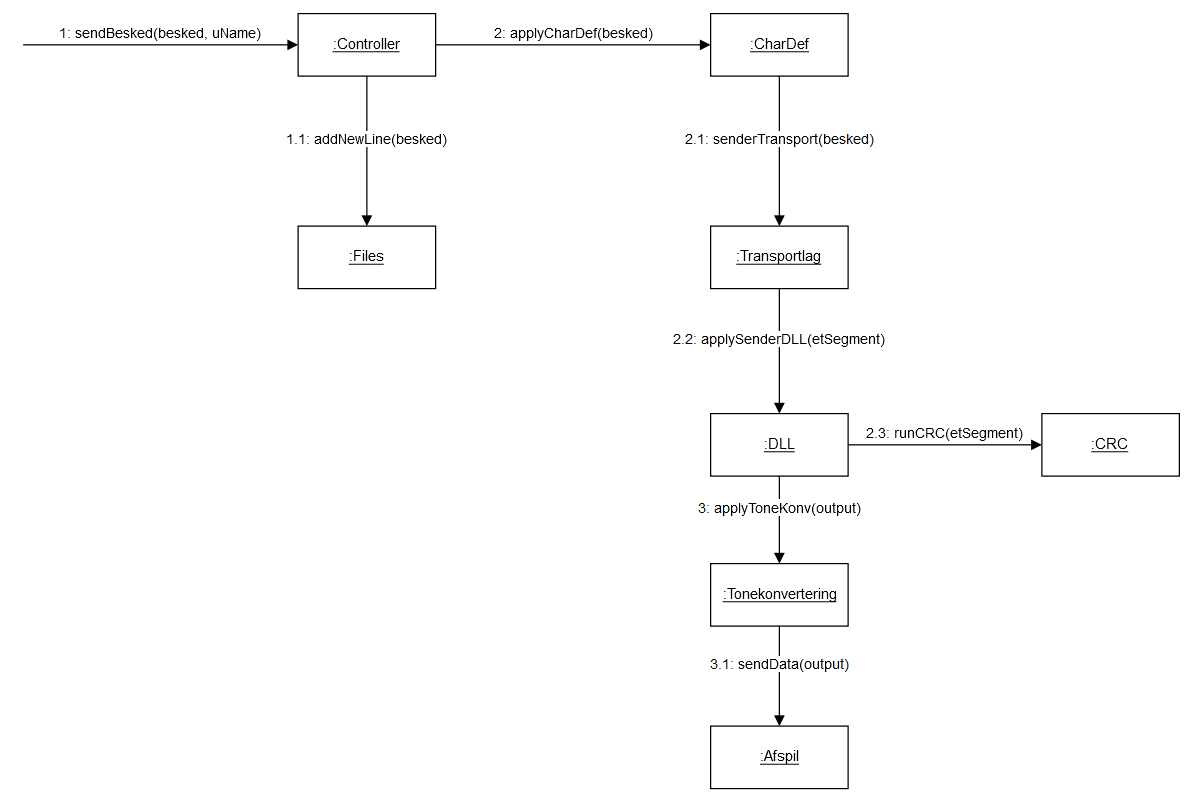
\includegraphics[width=15cm,height=25cm,keepaspectratio]{pictures/SDsend.png}
	\caption{\texttt{sendBesked()}}
	\label{fig:sendb}
\end{figure}
\hfill \break
Denne metode tager beskeden der skal sendes, samt navnet på den der har sendt den og samler det i en besked. Denne besked bliver sendt videre til \texttt{Chardefinition} klassen, som laver teksten om til en binær streng. Den bliver efterfølgende sendt til transportlaget, der kan dele beskeden op i mindre segmenter og sørge for at sendingerne foregår som de skal. Pakkerne vil kommere videre til Data Link Laget, hvor der vil blive tilføjet CRC og stuffing til bitstrengen. I \texttt{Tonekonvertering} bliver den binære streng omdannet til tal mellem 0 og 15, som er det antal toner der er til rådighed ved DTMF. Til sidst bliver tonerne afspillet med klassen \texttt{Afspil}. Når en besked er sendt, bliver den gemt i en fil med klassen \texttt{Files}.
\newline
Klassen har desuden en metode, der hedder \texttt{modtagBesked(uName)}. Samarbejdsdiagrammet for \texttt{modtagBesked()} er vist i figur \ref{fig:modtagb}.
\begin{figure}[ht]
	\centering
	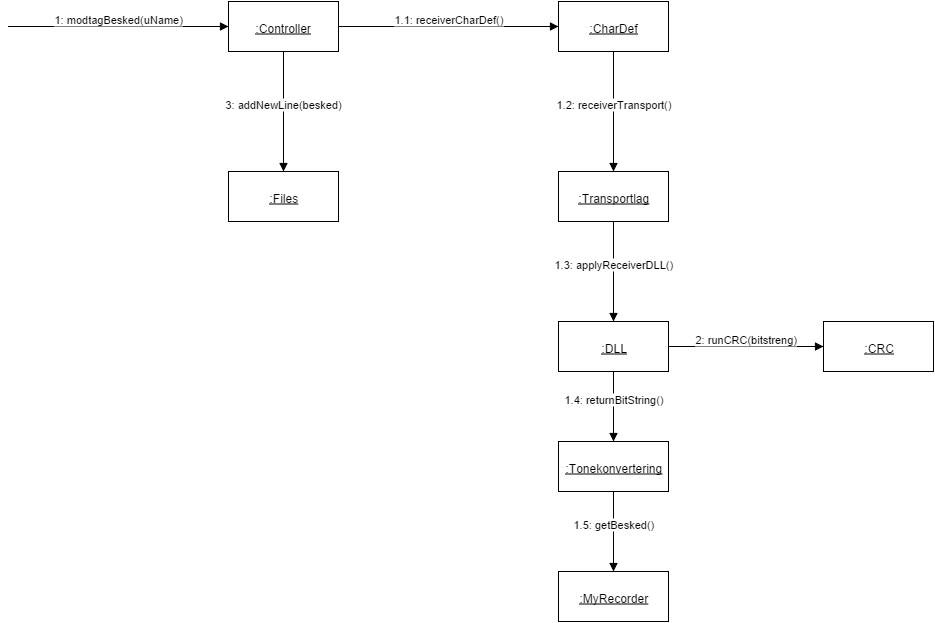
\includegraphics[width=15cm,height=25cm,keepaspectratio]{pictures/SDmodtagBesked.png}
	\caption{\texttt{modtagBesked()}}
	\label{fig:modtagb}
\end{figure}
\hfill \break
Denne går igennem de samme klasser som \texttt{sendBesked}, dog i stedet for at sende en besked afsted, sendes der en request om at modtage en besked. I klassen \texttt{MyRecorder} modtages beskeden, som returneres som toner af tal mellem 0 og 15 til \texttt{Tonekonvertering}'en, der omdanner tonerne til en bitstreng, som returneres til Data link laget. Ved \texttt{DLL} tjekkes for CRC og stuffing fjernes inden det returneres til transportlaget, hvor beskeden sættes sammen igen, hvis beskeden var delt op i segmenter. Den kommer retur til \texttt{CharDef} og bliver lavet fra binær streng til karakterer, som derefter returneres til \texttt{Controller}, der viser beskeden på skærmen og samtidig bruger \texttt{Files} til at gemme beskeden i en historik. Til dette bruges \texttt{uName} i metoden for at gemme i den rigtige historik.
\newline
\texttt{testLogin(uName, pWord)} er metoden der kan teste om et brugernavn og password er korrekt. Dette gør den ved at bruge \texttt{Login} klassen.
\newline
\texttt{createUser(uName, pWord)} bruger igen \texttt{Login} klassen, denne gang til at oprette en bruger. Samarbejddiagrammet er vist i figur \ref{fig:createu}.
\begin{figure}[ht]
	\centering
	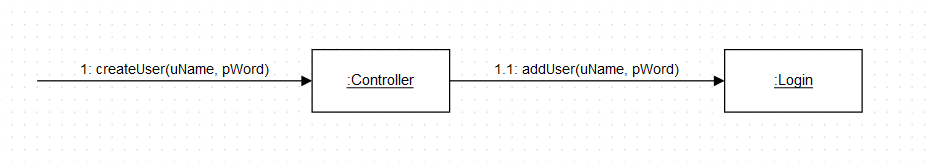
\includegraphics[width=15cm,height=25cm,keepaspectratio]{pictures/SDcreateUser.png}
	\caption{\texttt{createUser()}}
	\label{fig:createu}
\end{figure}
\hfill \break

Der er også metoder der kan vise historikken. De bruger alle \texttt{Files} klassen og kan enten vise hele historikken, sidste besked eller en der kan definere hvor mange linjer der skal hentes og vises.

\hfill \break
\underline{\textbf{Login klassen}}
\newline
Klassen \texttt{Login} bruges til at oprette og teste brugernavn og password. Metoden \texttt{addUser(uName, Pword)} opretter nye brugere og gemmer brugernavn og password i et txt dokument.
\newline
Klassen har også metoden \texttt{testLogin(uName, pWord)}, som bruger metoden \texttt{validateLogin(uName, pWord)}. Den modtager et brugernavn og login, som bliver lavet om til en string. Denne string bliver efterfølgende sammenlignet med alle de brugernavne og passwords der er gemt i txt filen. Hvis der ikke findes et match bliver der returneret true og brugeren logges på.

\hfill \break
\underline{\textbf{Files klassen}}
\newline
\texttt{Files} klassen bruges til at gemme historik, når der bliver skrevet til hinanden med chat programmet. Files virker ved at når der oprettes et objekt at klassen, med en parameter, som er brugernavnet, bliver der oprettet et txt dokument med brugerens navn, som historikken kan gemmes i.
\newline
Funktionen \texttt{addNewLine(besked)} tilføjer en besked til tekstdokumentet. \texttt{updateVector()} bruges til at lave en vektor af linjerne fra historikken, som efterfølgende evt. kan printes ud på en skærm så brugeren kan se indholdet. Der er en metode \texttt{clearText()}, der kan slette alt fra historikken. Der er også metoden \texttt{printVector()}, der kan printe hver linje ud, som er i vektoren skabt med \texttt{updateVector()}. \texttt{printLatest()} printer den sidste besked ud og \texttt{printLines(startN, endM)} kan printe de valgte linjer ud fra linje n til m. Til sidst er der en metoden flipVector(), den bruges til vende vectoren, så fx den sidste modtagne besked kommer til at ligge øverst i vektoren, altså på plads 0.

\hfill \break
\underline{\textbf{CharDefinition klassen}}
\newline
\texttt{CharDefinition} klassens opgave er at omdanne forskellige karakterer om til binærer tal og tilbage igen. Hvis der oprettes et objekt af klassen, bliver der skabt en string af alle de tal, karakterer og andre tegn der tænkes at skulle kunne sendes. Den string kan bruges i metoderne. Der er en metode som hedder \texttt{applyCharDef(input)}, der bruger en anden metode \texttt{charToBinary}, som kan omdanne karakterer i en besked til binær, inden den sendes videre til Tranportlaget.
\newline
\texttt{charToBinary(input)} metoden tager inputtet som er en string af karakterer og laver det om til en binær string. Det gør den ved at kigge på de karakterer, der skal sendes og sammenligne dem med de definerede karakterer og tegn. Hvis der findes et match, bruges nummeret på placeringen af karakteren i den definerede string, som den binære værdi. Den binære værdi bliver 8 bits lang. Fx karakteren b, som har placeringen 12, får binær værdien 00001100.
\newline
\texttt{receiverCharDef()} er metoden der bruges når der returneres beskeder fra transportlaget og laver beskeden om fra binær til karakterer. Hvis beskeden der modtages er en fejlbesked sende den videre og vises på skærmen. Ellers bruges metoden \texttt{binaryToChar(messageReceived)} der omdanner de otte bits om til et decimaltal, som igen kan bruges til at finde placeringen af karakteren, der er modtaget og derefter sætte det på en string. Det gøres indtil hele beskeden er omdannet.

\hfill \break
\underline{\textbf{UI source}}
\newline
Til chat programmet er der valgt at lave et simpelt user interface. Det blev lavet ved at bruge konsolvinduet i Visual Studio. Et flowdiagram af systemet er vist på figur \ref{fig:uif}.
\begin{figure}[ht]
	\centering
	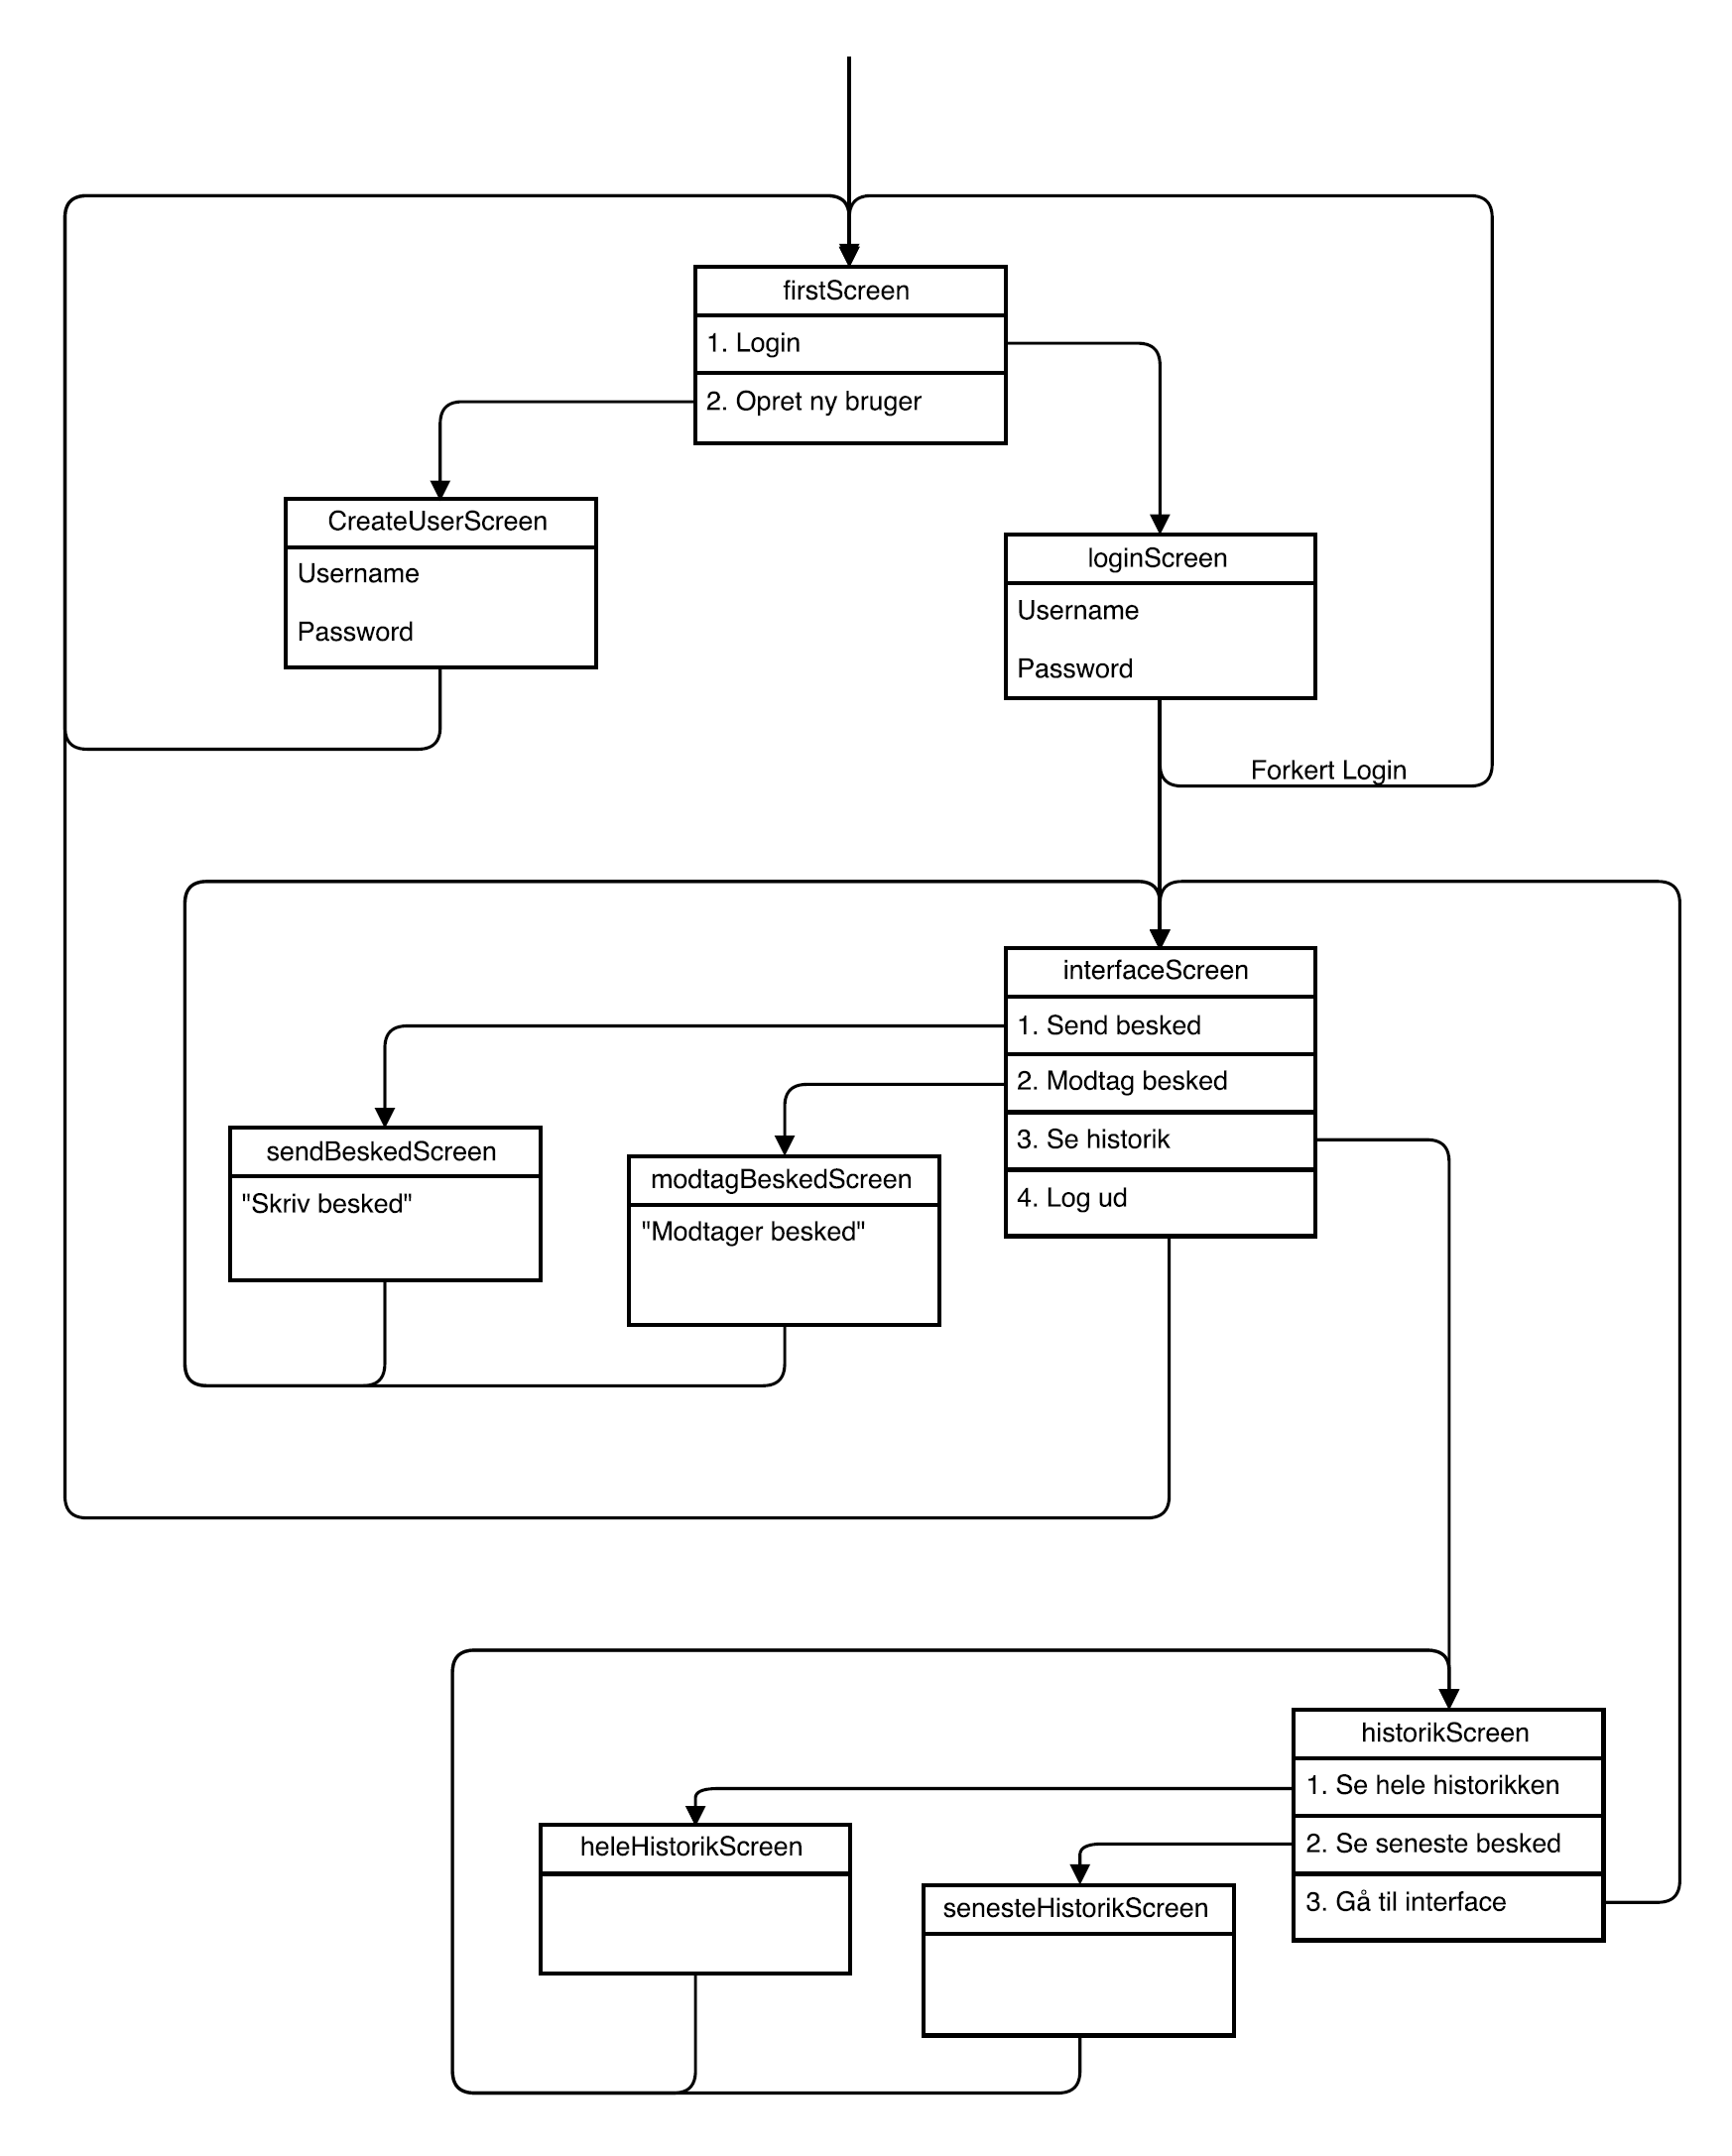
\includegraphics[width=15cm,height=25cm,keepaspectratio]{pictures/UIflow.png}
	\caption{\texttt{UI flowdiagram}}
	\label{fig:uif}
\end{figure}
Programmet er bygget op ved at der gives nogle valgmuligheder. På første skærm kan der vælges mellem login eller opret bruger. Der vælges ved at indtaste et tal, her 1 eller 2. Tallet sammenlignes med de muligheder der er og programmet går til næste skærm. Når der oprettes ny bruger, indtastes brugernavn og password som efterfølgende bruges i \texttt{Controller} klassen i metoden \texttt{createUser(uName, pWord)}. Der vil efterfølgende gås videre til loginskærmen, hvor brugernavn og password indtastes igen og bruges i metoden \texttt{testLogin(uName, pWord)}. Hvis det indtastede er forkert kan der prøves igen ellers kommer interface skærmen. Her er mulighederne: Send besked, modtag besked, se historik og log ud. Ved send besked skærmen kan der skrives en besked, som efterfølgende sendes med metoden \texttt{sendBesked(besked, uName)}. Ved modtagBesked skærmen afventes der en besked. Den modtages med metoden \texttt{modtagBesked()} og bliver efterfølgende vist på skærmen. Hvis der vælges historik, kommer en skærm med 3 muligheder igen. Her kan der vælges at se hele historikken eller seneste besked som vises med metoderne \texttt{getHeleHistory()} og \texttt{getSenesteHistory()}. Den sidste valgmulighed er retur til interface skærmen.
%	\input{subsections/TeoriKF}
%	\input{subsections/ProgrammeringKF}
	
%	\pagebreak
%	\input{sections/Random}
%	\pagebreak
%	\input{sections/Whatevs}
%	\pagebreak
%	\section{Konklusion}
Vi har ben
%	\pagebreak
%	\section{Perspektivering}
%	\pagebreak
	
%	\section{Litteraturliste}
\begingroup
\renewcommand{\section}[2]{}%

\begin{thebibliography}{1}
	\subsection{Bøger}
  \bibitem{notes} John W. Dower {\em Readings compiled for History
  21.479.}  1991.

  \bibitem{impj}  The Japan Reader {\em Imperial Japan 1800-1945} 1973:
  Random House, N.Y.
  
	\subsection{Hjemmesider}
  \bibitem{norman} E. H. Norman {\em Japan's emergence as a modern
  state} 1940: International Secretariat, Institute of Pacific
  Relations.

  \bibitem{fo} Bob Tadashi Wakabayashi {\em Anti-Foreignism and Western
  Learning in Early-Modern Japan} 1986: Harvard University Press.

  \end{thebibliography}
	
\end{document}